\subsection{UC5 - Visualizzazione degli indici di qualità delle previsioni sull'applicativo esterno}
\begin{figure}[H]
	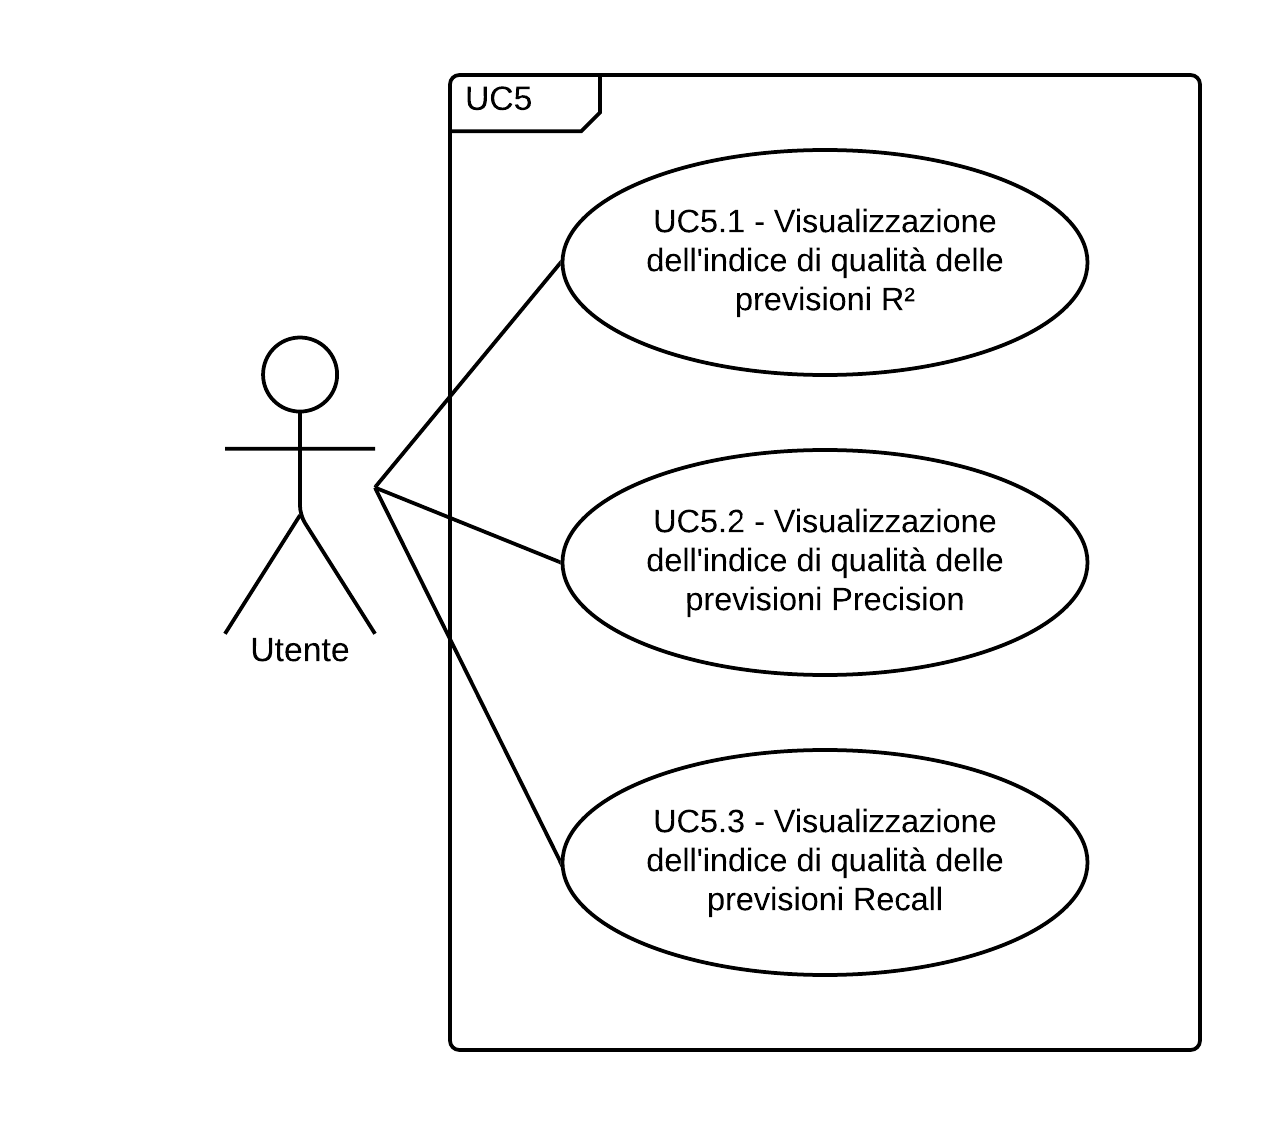
\includegraphics{img/UC5_-_Visualizzazione_degli_indici_di_qualita_delle_previsioni_sull'applicativo_esterno.png}
	\caption{Diagramma dello use case UC5}
\end{figure}
\begin{itemize}
	\item \textbf{Codice identificativo}: UC5;
	\item \textbf{Titolo}: visualizzazione degli indici di qualità delle previsioni;
	\item \textbf{Attori primari}: utente;
	\item \textbf{Descrizione}: l'utente visualizza gli indici numerici che rappresentano la misura di qualità delle previsioni sui dati forniti dall'addestramento;
	\item \textbf{Precondizioni}: l'addestramento è stato eseguito correttamente con l'applicazione esterna;
	\item \textbf{Postcondizioni}: l'utente ha visualizzato gli indici numerici di qualità delle previsioni;
	\item \textbf{Scenario principale}: l'utente visualizza gli indici numerici di qualità delle previsioni.
\end{itemize} 
\subsubsection{UC5.1 - Visualizzazione dell'indice di qualità delle previsioni R$^{2}$}
\begin{itemize}
	\item \textbf{Codice identificativo}: UC5.1;
	\item \textbf{Titolo}: visualizzazione dell'indice di qualità delle previsioni R$^{2}$\glo;
	\item \textbf{Attori primari}: utente;
	\item \textbf{Descrizione}: l'utente visualizza l'indice numerico che rappresenta la misura di qualità delle previsioni sui dati forniti attraverso il meccanismo R$^{2}$\glo;
	\item \textbf{Precondizioni}: l'addestramento è stato eseguito con l'applicazione esterna;
	\item \textbf{Postcondizioni}: l'utente ha visualizzato l'indice di qualità delle previsioni R$^{2}$\glo;
	\item \textbf{Scenario principale}: l'utente visualizza l'indice di qualità delle previsioni R$^{2}$\glo.
\end{itemize} 
\subsubsection{UC5.2 - Visualizzazione dell'indice di qualità delle previsioni Precision}
\begin{itemize}
	\item \textbf{Codice identificativo}: UC5.2;
	\item \textbf{Titolo}: visualizzazione dell'indice di qualità delle previsioni Precision\glo;
	\item \textbf{Attori primari}: utente;
	\item \textbf{Descrizione}: l'utente visualizza l'indice numerico che rappresenta la misura di qualità delle previsioni sui dati forniti attraverso il meccanismo Precision\glo;
	\item \textbf{Precondizioni}: l'addestramento è stato eseguito con l'applicazione esterna;
	\item \textbf{Postcondizioni}: l'utente ha visualizzato l'indice di qualità delle previsioni Precision\glo;
	\item \textbf{Scenario principale}: l'utente visualizza l'indice di qualità delle previsioni Precision\glo.
\end{itemize} 
\subsubsection{UC5.3 - Visualizzazione dell'indice di qualità delle previsioni Recall}
\begin{itemize}
	\item \textbf{Codice identificativo}: UC5.3;
	\item \textbf{Titolo}: visualizzazione dell'indice di qualità delle previsioni Recall\glo;
	\item \textbf{Attori primari}: utente;
	\item \textbf{Descrizione}: l'utente visualizza l'indice numerico che rappresenta la misura di qualità delle previsioni sui dati forniti attraverso il meccanismo Recall\glo;
	\item \textbf{Precondizioni}: l'addestramento è stato eseguito con l'applicazione esterna;
	\item \textbf{Postcondizioni}: l'utente ha visualizzato l'indice di qualità delle previsioni Recall\glo;
	\item \textbf{Scenario principale}: l'utente visualizza l'indice di qualità delle previsioni Recall\glo.
\end{itemize} 
